\documentclass[12pt, twoside]{article}
\usepackage[letterpaper, margin=1in, headsep=0.5in]{geometry}
\usepackage[english]{babel}
\usepackage[utf8]{inputenc}
\usepackage{amsmath}
\usepackage{amsfonts}
\usepackage{amssymb}
\usepackage{tikz}
%\usetikzlibrary{quotes, angles}

\usepackage{graphicx}
\usepackage{enumitem}
\usepackage{multicol}

\usepackage{fancyhdr}
\pagestyle{fancy}
\fancyhf{}
\renewcommand{\headrulewidth}{0pt} % disable the underline of the header

\fancyhead[RE]{\thepage}
\fancyhead[RO]{\thepage \\ Name: \hspace{3cm}}
\fancyhead[L]{BECA / Dr. Huson / 12.1 IB Math SL\\* 22 January 2019}

\begin{document}
\subsubsection*{Spiral Review: 6-1 P1 (No Calculator) Calculus Tangents}
 \begin{enumerate}

  \item 10N.1.sl.TZ0.2\\
  Let $g(x)=2x \sin x$.
  \begin{enumerate}
    \item Find $g'(x)$ [4 marks]
    \item Find the gradient of the graph of $g$ at $x=\pi$. [3 marks]
  \end{enumerate}

  \item 12M.1.sl.TZ1.3\\
  Let $f(x)=e^{6x}$.
  \begin{enumerate}
    \item Write down $f'(x)$ [1 mark]
    \item The tangent to the graph of $f$ at the point $P(0,b)$ has gradient $m$.  [4 marks]
    \begin{enumerate}
      \item Show that $m=6$.
      \item Find $b$.
    \end{enumerate}
    \item Hence, write down the equation of this tangent. [1 mark]
  \end{enumerate}

  \item 09M.1.sl.TZ1.3 [6 marks]\\
  Let $f(x)=e^{x} \cos x$. Find the gradient of the normal to the curve of $f$ at $x= \pi$.

  \item 13M.1.sl.TZ1.3\\
  Consider $f(x)=x^2 \sin x$.
  \begin{enumerate}
    \item Find $f'(x)$. [4 marks]
    \item Find the gradient of the curve of $f$ at $x= \frac{\pi}{2}$. [3 marks]
  \end{enumerate}

  \item 12N.1.sl.TZ0.4\\
  Part of the graph of $f(x)= ax^3-6x^2$ is shown below.
    \begin{center}
      \begin{tikzpicture}[scale=3]
        \draw [thick, ->] (-0.8,0) -- (1.8,0) node [below] {$x$};
        \draw [thick, ->] (0,-2) -- (0,0.5) node [left] {$y$};
        \draw[thick, domain=-0.45:1.25] plot[samples=100](\x, {5*(\x)^3 - 6*(\x)^2});
        \draw[dashed] (1,0)node[above]{$1$} --(1,-1) node[right]{P};
        \node at (1,-1) {\textbullet};
      \end{tikzpicture}
    \end{center}

    The point $P$ lies on the graph of $f$. At $P$, $x=1$.
    \begin{enumerate}
      \item Find $f'(x)$. [2 marks]
      \item The graph of $f$ has a gradient of 3 at the point $P$. Find the value of $a$. [4 marks]
    \end{enumerate}

  \item 17N.1.sl.TZ0.5\\
  Let $f(x)=1+e^{-x}$ and $g(x)=2x+b$, for $x \in \mathbb{R}$, where $b$ is a constant.
  \begin{enumerate}
    \item Find $(g \circ f)(x)$. [2 marks]
    \item Given that $\displaystyle \lim_{x \rightarrow +\infty} (g \circ f)(x) = -3$, find the value of $b$. [4 marks]
  \end{enumerate}

  \item 10M.1.sl.TZ2.5 [6 marks]\\
  Let $f(x)=kx^4$. The point $P(1,k)$ lies on the curve of $f$. At $P$, the normal to the curve is parallel to $y=- \frac{1}{8} x$. Find the value of $k$.

  \item 13N.1.sl.TZ0.6 [6 marks]\\
  Let $f(x)=e^{2x}$. The line $L$ is the tangent to the curve of $f$ at $(1,e^2)$.\\
  Find the equation of $L$ in the form $y=ax+b$.

  \item 17M.1.sl.TZ1.6\\
  The following diagram shows the graph of $f'$, the derivative of $f$.
    \begin{center}
      \begin{tikzpicture}[y=0.5cm]
        \draw [thick, ->] (-4,0) -- (10.5,0) node [below right] {$x$};
        \draw [thick, ->] (0,-12) -- (0,9) node [left] {$y$};
        \foreach \x in {-4,..., 10}
        \draw[shift={(\x,0)},color=black] (0pt,-3pt) -- (0pt,0pt) node[below=4pt]  {$\x$};
        \foreach \y in {-12,-10,...,8}
        \draw[shift={(0,\y)},color=black] (-3pt,0pt) -- (0pt,0pt) node[left=3pt]  {$\y$};

        \draw[thick, domain=-2:9] plot[samples=100](\x, {-0.104*(\x+0.9118)*(\x-6)^2});
        \draw [fill] (1.39,-5.09) circle [radius=0.05cm] node[below] {$A$};
        \draw [fill] (4,-2.01) circle [radius=0.05cm] node[below right]{$(4,-2)$};
        \draw [fill] (6,0) circle [radius=0.05cm] node[above] {$B$};
             %\draw[dashed] (1,0)node[above]{$1$} --(1,-1) node[right]{P};
      \end{tikzpicture}
    \end{center}

    The graph of $f'$ has a local minimum at $A$, a local maximum at $B$ and passes through $(4,2)$. The point $P(4,3)$ lies on the graph of the function, $f$.
    \begin{enumerate}
      \item Write down the gradient of the curve of $f$ at $P$. [1 mark]
      \item Find the equation of the normal to the curve of $f$ at $P$. [3 marks]
      \item Determine the concavity of the graph of $f$ when $4<x<5$ \textbf{and} justify your answer. [2 marks]
    \end{enumerate}

  \item 18M.1.sl.TZ1.7 [7 marks]\\
  Consider $f(x)$, $g(x)$ and $h(x)$, for $x \in \mathbb{R}$ where $h(x)=(f \circ g)(x)$.\\
  %Given that $g(3)=7$, $g'(3)=4$ and $f'(7)=−5$, find the gradient of the normal to the curve of $h$ at $x=3$.
  Given that $g(3)=7$, $g'(3)=4$, and $f'(7)=-5$, find the gradient of the normal to the curve of $h$ at $x=3$.


  \item 11M.1.sl.TZ2.8\\
  The following diagram shows part of the graph of the function $f(x)=2x^2$.
    \begin{center}
      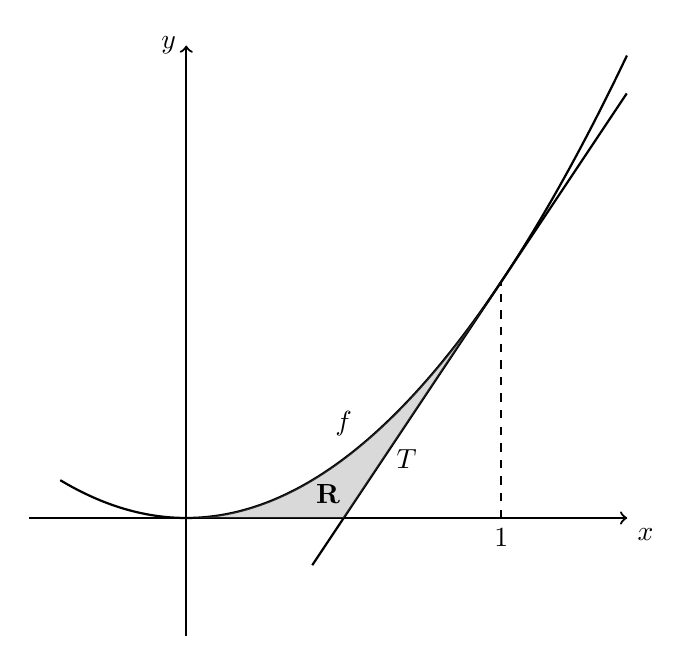
\begin{tikzpicture}[xscale=4, yscale=1.5]
        \draw [thick, ->] (-0.5,0) -- (1.4,0) node [below right] {$x$};
        \draw [thick, ->] (0,-1) -- (0,4) node [left] {$y$};
        \draw[thick] plot[samples=100, domain=0.4:1.4](\x, {4*\x-2});
        \draw[thick, domain=-0.4:1.4] plot[samples=100](\x, {2*\x*\x});
        \fill[gray,opacity=.3] (0.5,0)--plot[domain=0:1](\x, {2*\x*\x});
        \draw[thick, dashed] (1,0) node[below]{$1$} --(1,2);
        \draw (0.7,0.5) node {$T$};
        \draw (0.45,0.2) node {$\mathbf{R}$};
        \draw (0.5,0.8) node {$f$};
      \end{tikzpicture}
    \end{center}

    The line T is the tangent to the graph of $f$ at $x=1$.
    \begin{enumerate}
      \item Show that the equation of $T$ is $y=4x-2$. [5 marks]
      \item Find the $x$-intercept of $T$. [2 marks]
      \item The shaded region $R$ is enclosed by the graph of $f$, the line $T$, and the $x$-axis. [9 marks]
      \begin{enumerate}
        \item Write down an expression for the area of $R$.
        \item Find the area of $R$.
      \end{enumerate}
    \end{enumerate}


    \item 08M.1.sl.TZ1.8\\
    Consider $f(x)= \frac{1}{3} x^3+2x^2-5x$. Part of the graph of $f$ is shown below. There is a maximum point at $M$, and a point of inflexion at $N$.
      \begin{center}
        \begin{tikzpicture}[xscale=0.8, yscale=0.15]
          \draw [thick, ->] (-8.3,0) -- (4,0) node [below] {$x$};
          \draw [thick, ->] (0,-4) -- (0,40) node [left] {$y$};
          \draw[thick, domain=-7:3] plot[samples=100](\x, {0.333*(\x)^3 +2*(\x)^2-5*\x});
          \node at (-5,33.333){\textbullet};
          \node at (-5,33.333)[above]{$M$};
          \node at (-2,15.333){\textbullet};
          \node at (-2,15.333)[right]{$N$};
        \end{tikzpicture}
      \end{center}
      \begin{enumerate}
        \item Find $f'(x)$. [3 marks]
        \item Find the x-coordinate of $M$. [4 marks]
        \item Find the x-coordinate of $N$. [3 marks]
        \item The line $L$ is the tangent to the curve of $f$ at $(3,12)$. Find the equation of $L$ in the form $y=ax+b$. [4 marks]
      \end{enumerate}

    \item 17M.1.sl.TZ1.9\\
    A quadratic function $f$ can be written in the form  $f(x)=a(x-p)(x-3)$. The graph of $f$ has an axis of symmetry $x=2.5$ and $y$-intercept at $(0,-6)$.
    \begin{enumerate}
      \item Find the value of $p$. [3 marks]
      \item Find the value of $a$. [3 marks]
      \item The line $y=kx-5$ is a tangent to the curve of $f$. Find the values of $k$. [8 marks]
    \end{enumerate}

    \item 15M.1.sl.TZ1.9\\
    A function $f$ has its derivative given by $f'(x)=3x^2-2kx-9$, where $k$ is a constant.
    \begin{enumerate}
      \item Find $f''(x)$. [2 marks]
      \item The graph of $f$ has a point of inflexion when $x=1$.\\
      Show that $k=3$. [3 marks]
      \item Find $f'(-2)$. [2 marks]
      \item Find the equation of the tangent to the curve of $f$ at $(-2,1)$, giving your answer in the form  $y=ax-b$. [4 marks]
      \item Given that $f'(-1)=0$, explain why the graph of $f$ has a local maximum when $x=-1$. [3 marks]
    \end{enumerate}

    \item 13M.1.sl.TZ2.9\\
    Let $f(x)=\sin x + \frac{1}{2} x^2 -2x$, for $0 \leq x \leq \pi$.
    \begin{enumerate}
      \item Find $f'(x)$. [3 marks]
      \item Let $g$ be a quadratic function such that $g(0)=5$. The line $x=2$ is the axis of symmetry of the graph of $g$.\\
      Find $g(4)$. [3 marks]
      \item The function $g$ can be expressed in the form $g(x)=a(x-h)^2+3$.
        \begin{enumerate}
          \item Write down the value of $h$.
          \item Find the value of $a$.
        \end{enumerate}
      \item Find the value of $x$ for which the tangent to the graph of $f$ is parallel to the tangent to the graph of $g$. [6 marks]
    \end{enumerate}

    \item 11N.1.sl.TZ0.9\\
    The following diagram shows the graph of $f(x)=a \sin (b(x-c))+d$, for $2 \leq x \leq 10$.
      \begin{center}
        \begin{tikzpicture}[x=0.6cm, y=0.5cm]
          \draw [thick, ->] (-1,0) -- (12,0) node [below right] {$x$};
          \draw [thick, ->] (0,-5) -- (0,14) node [left] {$y$};
          \foreach \x in {0,5, 10}
          \draw[shift={(\x,0)},color=black] (0pt,-3pt) -- (0pt,0pt) node[below=4pt]  {$\x$};
          \foreach \y in {-5,0,5,10}
          \draw[shift={(0,\y)},color=black] (-3pt,0pt) -- (0pt,0pt) node[left=3pt]  {$\y$};

          \draw[thick, domain=2:10] plot[samples=100](\x, {8*sin(deg(3.14159*(\x-2)/4)) +4});
          \draw [fill] (4,12) circle [radius=0.05cm] node[above] {$P(4,12)$};
          \draw [fill] (8,-4) circle [radius=0.05cm] node[below]{$Q(8,-4)$};
        \end{tikzpicture}
      \end{center}
      There is a maximum point at $P(4,12)$ and a minimum point ast $Q(8, -4)$.
      \begin{enumerate}
        \item Use the graph to write down the value of [3 marks]
          \begin{enumerate}
            \item $a$;
            \item $c$;
            \item $d$.
          \end{enumerate}
        \item Show that $b= \frac{\pi}{4}$. [2 marks]
        \item Find $f'(x)$. [3 marks]
        \item At a point $R$, the gradient is $-2 \pi$. Find the $x$-coordinate of $R$. [6 marks]
      \end{enumerate}

    \item 16M.1.sl.TZ1.10 \hfill [15 marks]\\
    Let $f(x)=\sqrt{4x+5}$, for $x \geq -1.25$.
    \begin{enumerate}
      \item Find $f'(1)$. \hfill [4]
      \item Consider another function $g$. Let $R$ be a point on the graph of $g$. The $x$-coordinate of $R$ is 1. The equation of the tangent to the graph at $R$ is  $y=3x+6$.\\
      Write down $g'(1)$. \hfill [2]
      \item Find $g(1)$. \hfill [2]
      \item Let $h(x)=f(x) \times g(x)$. Find the equation of the tangent to the graph of $h$ at the point where $x=1$. \hfill [7]
    \end{enumerate}

\end{enumerate}
\end{document}
